% IE 643 Novelty Assessment report (max. 2 pages) -- Team Gradient Mavericks
% Header macro from the official IE643_2026_Report_template. Condensed from ../IE643_Project_Report.tex.
% Compile:  tectonic Gradient_Mavericks_IE643_NoveltyAssessment_report.tex
\documentclass[10pt]{article}
\usepackage[a4paper,left=0.6in,right=0.6in,top=0.5in,bottom=0.55in]{geometry}
\usepackage{amsmath,amssymb,graphicx,booktabs,xcolor,enumitem,caption}
\usepackage[hidelinks]{hyperref}
\captionsetup{font=footnotesize,labelfont=bf,skip=2pt}
\setlength{\parindent}{0in}
\setlength{\parskip}{2pt}
\setlist{nosep,leftmargin=12pt}
\setlength{\textfloatsep}{5pt}
\setlength{\abovedisplayskip}{2pt}\setlength{\belowdisplayskip}{2pt}
\setlength{\abovedisplayshortskip}{1pt}\setlength{\belowdisplayshortskip}{1pt}
\graphicspath{{../figs/}}
\pagestyle{plain}

\newcommand{\lecture}[3]{
   \begin{center}
   \framebox{\vbox{\vspace{1mm}
    \hbox to \dimexpr\textwidth-0.25in\relax{{\bf IE 643: Deep Learning - Theory and Practice \hfill July-Dec 2026}}
    \vspace{2mm}
    \hbox to \dimexpr\textwidth-0.25in\relax{\parbox{\dimexpr\textwidth-0.25in\relax}{\centering\large Novelty Assessment Report: #1}}
    \vspace{2mm}
    \hbox to \dimexpr\textwidth-0.25in\relax{{\it Team Name: #2 \hfill Team Members: #3}}
    \vspace{1mm}}}
   \end{center}\vspace{-2mm}}
\newcommand{\hx}{\hat{x}_0}
\newcommand{\sect}[1]{\vspace{2pt}{\large\bf #1}\par}

\begin{document}
\lecture{Classifier- and Adversarially-Guided LoRA Fine-Tuning of Stable Diffusion for Rare-Pathology Chest X-rays}{Gradient Mavericks}{Saksham Jain (23B1074), Somya Dahiaya (23B1025)}

\sect{1\quad Starting point and review feedback}
In the intensive phase we LoRA~[2]-fine-tuned a CXR-adapted Stable Diffusion 1.5 (``P-Rajiv'') on 4{,}401 frontal CheXpert~[1] images with the denoising loss only, and added 2{,}173 synthetic images of five rare classes (Enlarged Cardiomediastinum, Lung Lesion, Pneumonia, Pleural Other, Fracture) to a 14-class DenseNet-121. Augmentation \emph{hurt}. The review asked for (i)~a classifier (CE) signal during LoRA training, compared with P-Rajiv; (ii)~per-pathology rates of ``shows the requested finding'' and ``structural defects''; (iii)~DenseNet with/without synthetic data on the same held-out real test set, per pathology; (iv)~model selection by validation metrics, not loss curves. We also wanted a loss for \emph{how real} images look.

\sect{2\quad Approaches tried}
\textbf{Image-level losses on a differentiable sample.} Following ReFL~[3], we run DDIM+CFG from noise \emph{without} gradient to a random late step $t_k\in[50,400]$, take one UNet step \emph{with} gradient, form $\hat z_0=(z_{t_k}-\sqrt{1-\bar\alpha_{t_k}}\,\hat\epsilon_\theta)/\sqrt{\bar\alpha_{t_k}}$ and decode $\hx$. Its features $f=\phi(\hx)$ come from a frozen TorchXRayVision~[4] DenseNet-121 (\texttt{res224-all}). Gradients reach the UNet and text-encoder LoRAs:
\begin{equation*}
L_G=L_{\text{diff}}+\lambda_{\text{cls}}\,L_{\text{cls}}(h_{\text{cls}}(f),y)+\lambda_{\text{adv}}\,\big(-D(f,y)\big),\qquad \lambda_{\text{cls}}=0.1,\ \lambda_{\text{adv}}=0.05 .
\end{equation*}
\begin{itemize}
\item \textbf{Classifier loss} ($h_{\text{cls}}$: frozen 6-class linear head fitted on real images). \emph{CE} (instructor's signal) never saturates, so it rewards ever more confident, exaggerated images. \textbf{Proposed: matched-confidence margin} $L_{\text{margin}}=\max(0,\,m_y-[s_y-\max_{k\neq y}s_k])$~[5], where $m_y$ is the median margin of correctly classified \emph{real} images of class $y$: the loss stops once an image is as recognisable as a typical real X-ray.
\item \textbf{Adversarial loss.} A class-conditional projection discriminator~[6] $D(f,y)=w^\top h(f)+e_y^\top h(f)$ (spectral norm, hinge loss, 200-step warm-up) on the frozen features. \textbf{Noise-level-matched real reference:} real latents are noised to the same $t_k$ and passed through the same one-step estimate, so $D$ cannot win by detecting one-step blur.
\item \textbf{Ablations/variants:} \emph{control} (2k extra steps, no new loss); CE-only; Adv-only ($\lambda_{\text{adv}}{=}0.05, 0.2$); CE+Adv; Margin+Adv; \textbf{multi-scale $D$} (Projected-GAN~[7] patch heads on 3 DenseNet stages); tuned guidance (CFG 4, LoRA scale 0.75); CheXpert-style JPEG/size matching; DA-Fusion img2img~[8] from real images.
\item \textbf{Downstream ``recipe''}: class weights from real counts only, synthetic loss weight 0.5, last 3 of 10 epochs on real only; optional filtering by reward margin + anatomy check.
\end{itemize}
\textbf{Held-out evaluation (no judge is a training signal).} \emph{Requested-finding rate}: a 6-class probe on a \emph{different} backbone, TorchXRayVision \texttt{mimic\_ch} (MIMIC-only, so no CheXpert leakage); 29.7\% accurate on real test images (chance 16.7\%), so we also report the rate normalised by its real-image recall. \emph{Structural defect} = PSPNet anatomy check fails (one left/right lung, plausible lung/heart areas, correct sides; 95.7\% of real images pass) \textbf{or} OOD (Mahalanobis distance~[9] above the 95th percentile of real validation images; 1.7\% of real flagged). Also KID~[10] per class. \textbf{Checkpoint selection}: every 500 steps a fixed seed grid is scored and the step maximising (requested-finding $-$ defect) is kept. \textbf{Protocol fix}: the original DenseNet script selected epochs on the \emph{test} set; we moved this to a patient-level validation split and train every setting with 3 seeds.

\sect{3\quad Experiments and results}
Setup: 2{,}000 LoRA steps per run (AdamW $2{\times}10^{-5}$, batch 4 + reward batch 2), one RTX A6000 each; 2{,}173 images per generator; DenseNet-121 on 16.6k real images, tested on 700 real images (50/class). In total \textbf{10 generators and 19 downstream settings $\times$ 3 seeds (57 runs)}.

\begin{table}[h]
\centering\footnotesize
\caption{Generation quality by held-out judges, mean over the 5 target classes (2{,}173 images per generator). Norm.\ cond.\ $=1$: as recognisable as real; $>1$: exaggerated.}\label{tab:gen}
\begin{tabular}{@{}lcccccc@{}}
\toprule
Generator ($\lambda_{\text{cls}}$, $\lambda_{\text{adv}}$; selected step) & Req.\ finding $\uparrow$ & Norm.\ cond. & Defects $\downarrow$ & OOD & KID$\times10^3\downarrow$ & Diversity\\
\midrule
P-Rajiv LoRA (phase-1 baseline) & 15.7\% & 0.56 & 32.7\% & 28.7\% & 12.8 & 0.257\\
Control: +2k steps, no new loss & 23.6\% & 0.89 & 51.8\% & 44.4\% & 10.3 & 0.318\\
CE only (0.1, 0; 1000, stopped) & 35.3\% & 1.29 & 78.5\% & 68.0\% & 29.9 & 0.219\\
Adversarial only (0, 0.05; 2000) & 25.9\% & 0.85 & 9.8\% & 7.2\% & 2.9 & 0.256\\
CE + adversarial (0.1, 0.05; 1000) & 45.9\% & 1.57 & 24.6\% & 18.3\% & 8.2 & 0.231\\
\textbf{Margin + adversarial} (0.1, 0.05; 1500) & \textbf{51.2\%} & 1.87 & 18.2\% & 12.9\% & 7.8 & 0.262\\
Margin + adv, multi-scale $D$ (1000) & 43.8\% & 1.57 & 16.5\% & 11.8\% & 8.7 & 0.248\\
DA-Fusion img2img from real (CE+adv LoRA) & 39.4\% & 1.38 & 10.4\% & 5.0\% & 3.0 & 0.322\\
\midrule
Real test images (reference) & 29.7\% & 1.00 & 4.3\%$^\ast$ & 1.7\% & -- & 0.345\\
\bottomrule
\end{tabular}\\[1pt]
{\scriptsize $^\ast$anatomy-check failure rate of real test images.}
\end{table}

\begin{minipage}[t]{0.47\textwidth}\vspace{0pt}
\centering
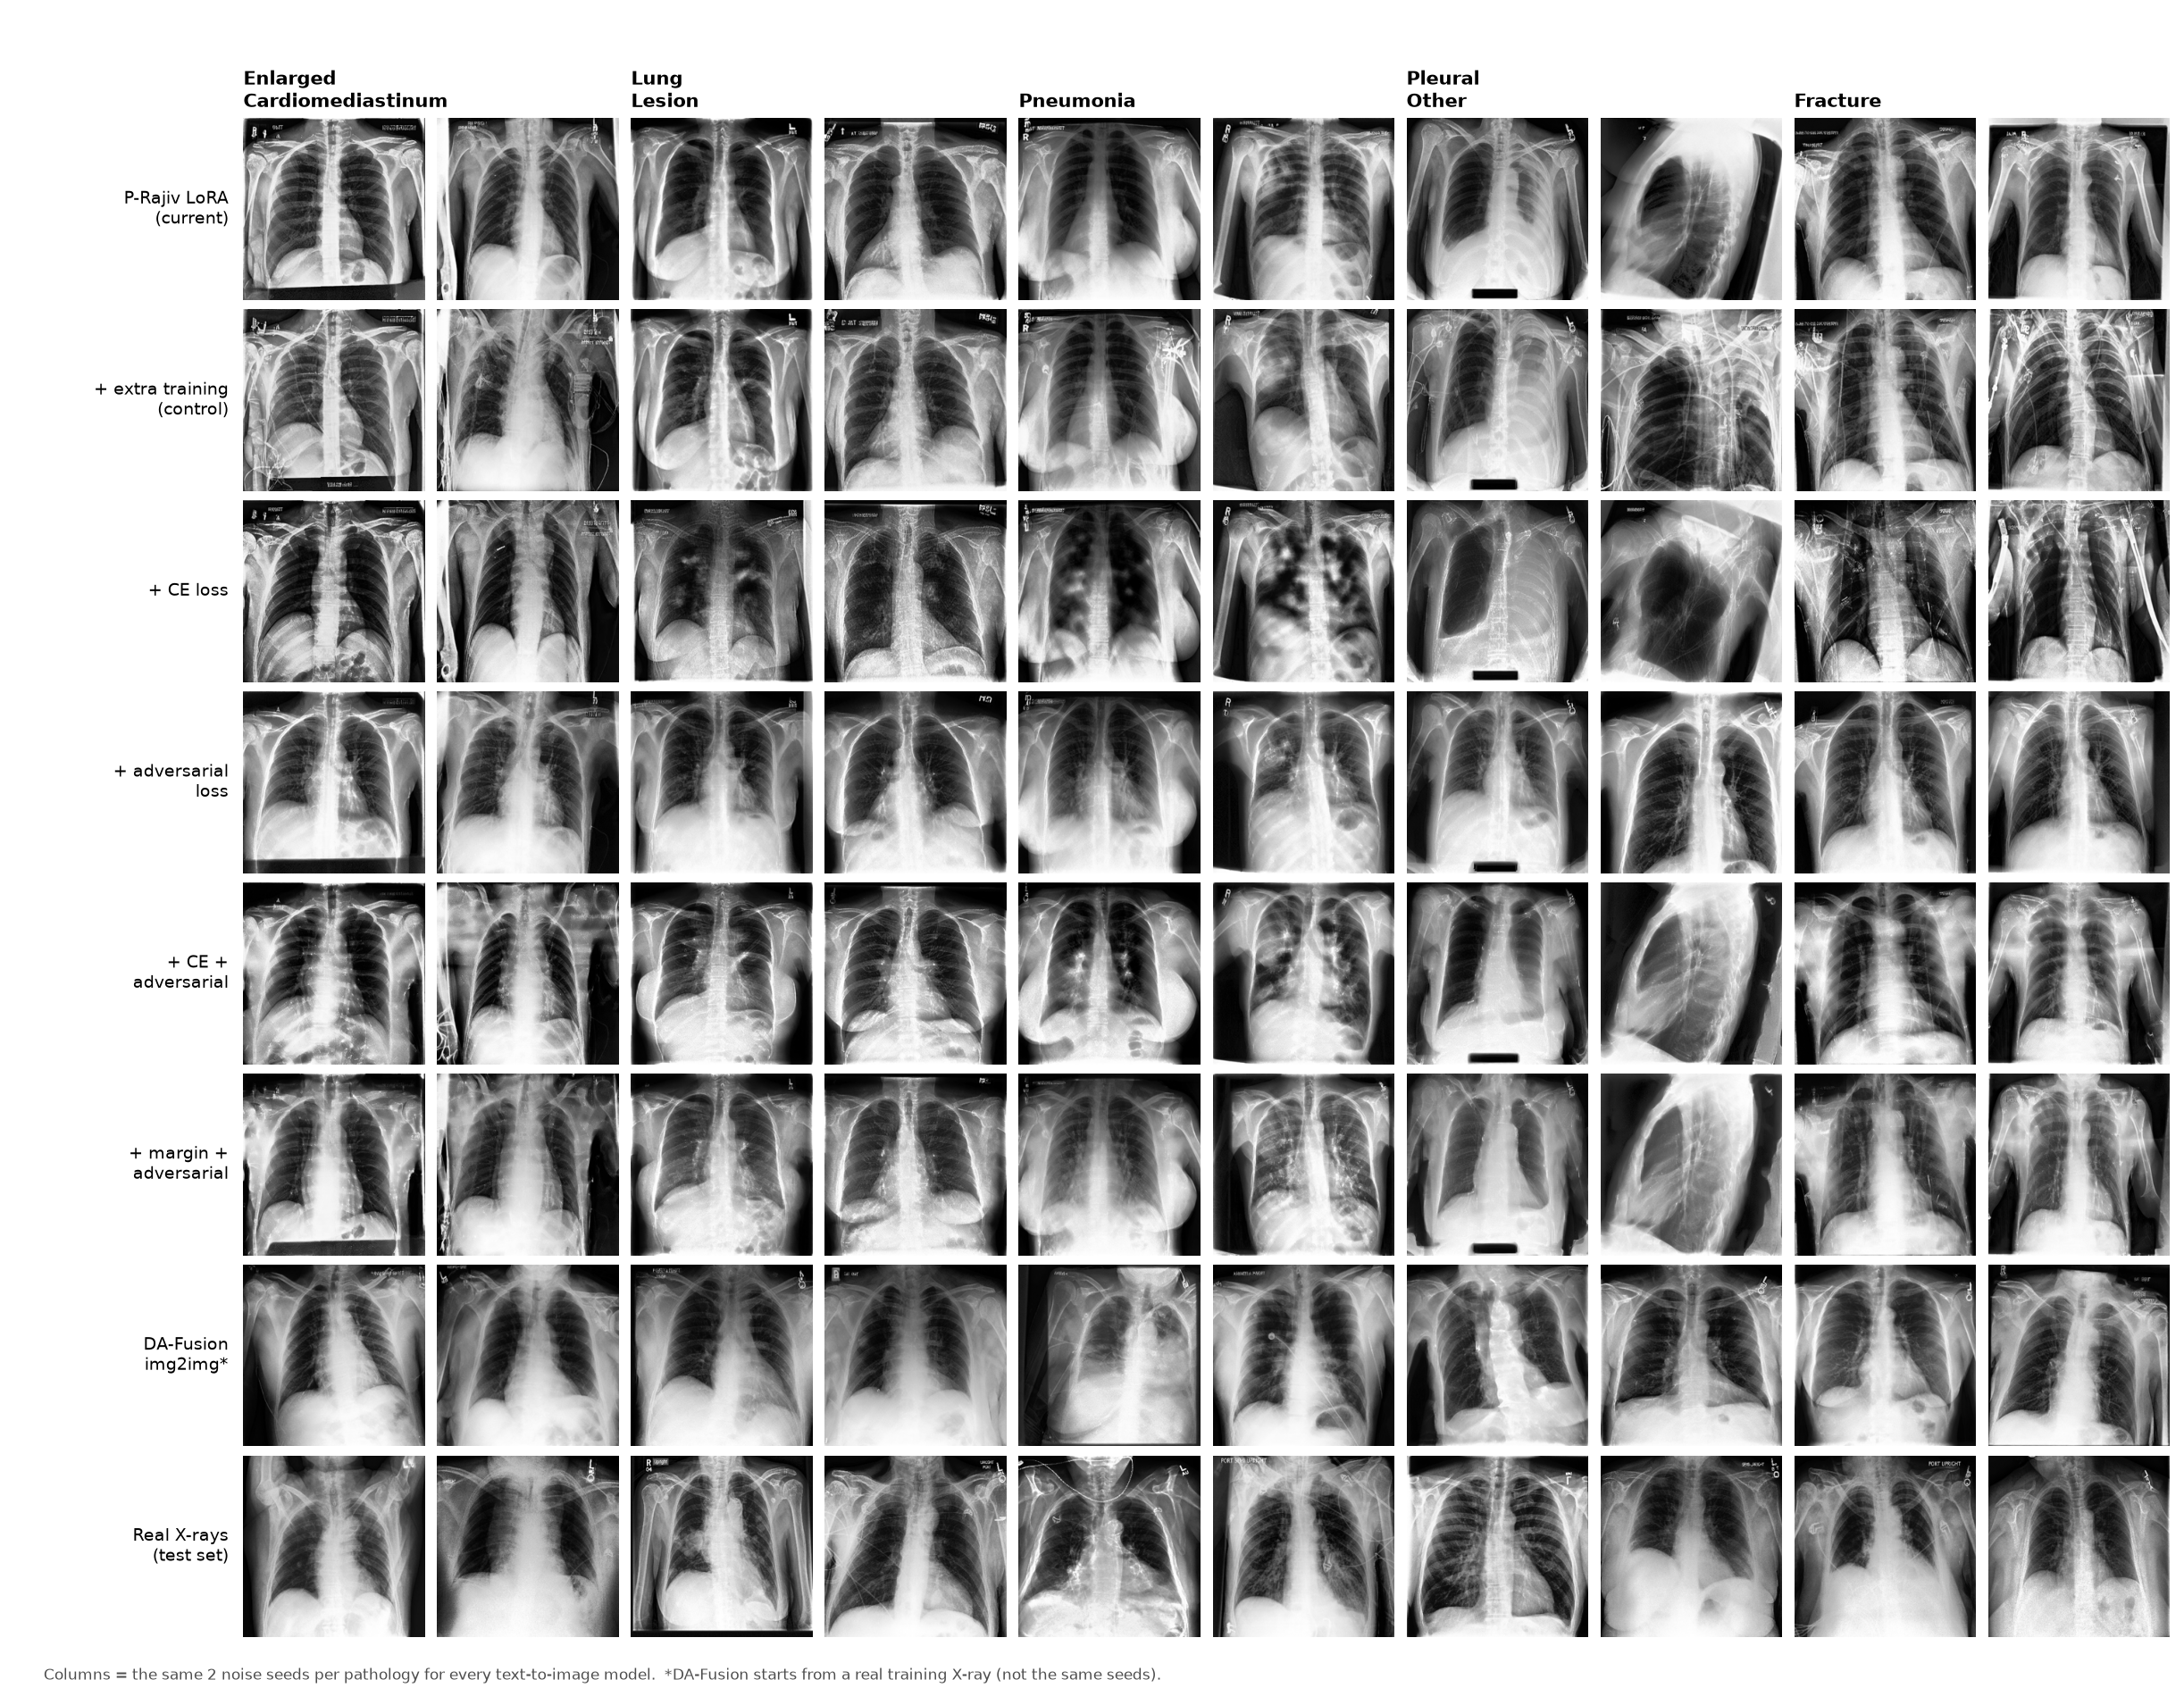
\includegraphics[width=\linewidth,trim=0 0 0 0,clip]{fig_samples_same_seeds.png}
\captionof{figure}{Same noise seeds across generators. CE-only gives blotchy textures (reward hacking); Adv-only is clean but generic; Margin+Adv shows findings with intact anatomy.}\label{fig:samples}
\end{minipage}\hfill
\begin{minipage}[t]{0.515\textwidth}\vspace{0pt}
\centering\footnotesize
\captionof{table}{Downstream 14-class DenseNet-121, test F1 on the same 700 real images (mean of 3 seeds; macro-F1 $\pm$ std). EC, LL, Pn, PO, Fr = generated classes. [r] = recipe.}\label{tab:ds}
\setlength{\tabcolsep}{2.5pt}
\begin{tabular}{@{}lcccccc@{}}
\toprule
Training data & Macro-F1 & EC & LL & Pn & PO & Fr\\
\midrule
\textbf{Real only} & \textbf{.285}$\pm$.012 & \textbf{.311} & .264 & .204 & .198 & .286\\
+ P-Rajiv baseline & .256$\pm$.013 & .237 & .210 & .102 & .112 & .287\\
+ CE only & .258$\pm$.017 & .235 & .247 & .152 & .105 & .313\\
+ Margin+Adv & .278$\pm$.008 & .271 & \textbf{.281} & .148 & .049 & \textbf{.358}\\
+ CE+Adv [r] & .283$\pm$.015 & .236 & .217 & .233 & .134 & .334\\
+ Margin+Adv [r] & .279$\pm$.007 & .281 & .256 & .207 & .154 & .342\\
+ Multi-scale $D$ [r] & .281$\pm$.019 & .277 & .237 & \textbf{.240} & \textbf{.200} & .297\\
+ DA-Fusion [r+filter] & .279$\pm$.012 & .239 & .262 & .223 & .152 & .284\\
\bottomrule
\end{tabular}
\end{minipage}

\vspace{4pt}
\textbf{Key findings.}
\begin{itemize}
\item \textbf{Only the combination improves both axes.} Margin+Adv raises the requested-finding rate $3.3\times$ (15.7$\to$51.2\%) while cutting defects (32.7$\to$18.2\%) and KID (12.8$\to$7.8). The control \emph{increases} defects (51.8\%), so the gains come from the new losses, not from extra training.
\item \textbf{The CE signal alone reward-hacks}: defects rose from 44\% to 87\% within 1{,}000 steps (KID 29.9). The margin loss and the adversarial term keep images on the real-image manifold. \textbf{Realism alone does not condition}: Adv-only has 9.8\% defects but follows the prompt only 25.9\% of the time; $\lambda_{\text{adv}}=0.2$ is worse (17.8\%).
\item \textbf{Multi-scale $D$ is a trade-off}: fewer defects (16.5\%) and less exaggeration, but weaker conditioning (43.8\%). \textbf{Checkpoint selection matters}: CE-based runs peak at 1{,}000--1{,}500 steps and then degrade, which loss curves do not show.
\item \textbf{Downstream: parity, not improvement.} The original augmentation lowered macro-F1 (0.285$\to$0.256); new generators + recipe reach 0.283$\pm$0.015, within seed noise of real-only. \textbf{Fracture} improves with the combined-loss generators (+0.05 to +0.07) and Pneumonia with CE+Adv and multi-scale $D$ [r] (+0.03); Pleural Other (241 real images) drops in every synthetic setting except multi-scale $D$ [r]. \emph{How} synthetic data is used mattered as much as image quality, and image metrics did not predict usefulness.
\end{itemize}

\sect{4\quad Why no overall gain, and next steps}
This matches prior work~[11]: synthetic data helps mainly when real data is scarce or the test set is shifted. Our generator is trained on the same CheXpert images and labels the classifier sees (no new information), the task is capped by label noise (even the probe is 29.7\% on real images), and differences below $\approx$0.02 macro-F1 are within noise (50 test images/class, 3 seeds). \textbf{Limitations}: classifier-based judges, not radiologists; reward and judge share the DenseNet-121 architecture; six template prompts; one seed per LoRA. \textbf{Next}: low-data (10--25\% real) and shifted-test (MIMIC/NIH) studies; multi-step reward gradients (DRaFT~[12]) with a KL penalty; rewarding downstream usefulness directly. \textbf{Code}: \url{https://github.com/somyadahiaya/ie643-cxr-diffusion}.

\vspace{2pt}
{\scriptsize\textbf{References.}
[1] Jeremy Irvin, Pranav Rajpurkar, Michael Ko et al. CheXpert: A Large Chest Radiograph Dataset with Uncertainty Labels and Expert Comparison, AAAI, 2019. https://arxiv.org/abs/1901.07031\;
[2] Edward J. Hu, Yelong Shen, Phillip Wallis et al. LoRA: Low-Rank Adaptation of Large Language Models, ICLR, 2022. https://arxiv.org/abs/2106.09685\;
[3] Jiazheng Xu, Xiao Liu, Yuchen Wu et al. ImageReward: Learning and Evaluating Human Preferences for Text-to-Image Generation, NeurIPS, 2023. https://arxiv.org/abs/2304.05977\;
[4] Joseph Paul Cohen, Joseph D. Viviano, Paul Bertin et al. TorchXRayVision: A Library of Chest X-ray Datasets and Models, MIDL, 2022. https://arxiv.org/abs/2111.00595\;
[5] Koby Crammer and Yoram Singer. On the Algorithmic Implementation of Multiclass Kernel-based Vector Machines, JMLR, 2001. https://www.jmlr.org/papers/v2/crammer01a.html\;
[6] Takeru Miyato and Masanori Koyama. cGANs with Projection Discriminator, ICLR, 2018. https://arxiv.org/abs/1802.05637\;
[7] Axel Sauer, Kashyap Chitta, Jens M\"uller and Andreas Geiger. Projected GANs Converge Faster, NeurIPS, 2021. https://arxiv.org/abs/2111.01007\;
[8] Brandon Trabucco, Kyle Doherty, Max Gurinas and Ruslan Salakhutdinov. Effective Data Augmentation With Diffusion Models, ICLR, 2024. https://arxiv.org/abs/2302.07944\;
[9] Kimin Lee, Kibok Lee, Honglak Lee and Jinwoo Shin. A Simple Unified Framework for Detecting Out-of-Distribution Samples and Adversarial Attacks, NeurIPS, 2018. https://arxiv.org/abs/1807.03888\;
[10] Miko{\l}aj Bi\'nkowski, Danica J. Sutherland, Michael Arbel and Arthur Gretton. Demystifying MMD GANs, ICLR, 2018. https://arxiv.org/abs/1801.01401\;
[11] Suman Ravuri and Oriol Vinyals. Classification Accuracy Score for Conditional Generative Models, NeurIPS, 2019. https://arxiv.org/abs/1905.10887\;
[12] Kevin Clark, Paul Vicol, Kevin Swersky and David J. Fleet. Directly Fine-Tuning Diffusion Models on Differentiable Rewards, ICLR, 2024. https://arxiv.org/abs/2309.17400
\par}
\end{document}
